\documentclass{td}

\usepackage{src/sty/config}

\codeUE{XLG4IU020}
\intituleUE{Programmation Concurrente en Multi-Threads}
\cursus{M1 ALMA \& Smart Computing}

\author{Matthieu \textsc{Perrin}}

\logo{src/img/logoUN.png}
\institution{Nantes Université}

\typeTP[3]
\title{Parallélisation de calcul d'image}

\hypersetup{
  pdftitle  = {TP 3 - Parallélisation de calcul d'image},
  pdfauthor = {Matthieu Perrin},
  pdfsubject  = {TP de M1 du cours Programmation Concurrente en Multi-Threads},
  pdfkeywords = {concurrence, Java, modèle de mémoire, moniteur, parallélisme, sûreté, thread, verrou, vivacité}
}

\begin{document}

\maketitle

Le but de ce travail est de paralléliser un programme affichant une représentation
graphique de l'ensemble de Mandelbrot. Une grande portion du code a déjà été faite pour vous.

Le code de départ est disponible sur le dépôt GitHub du cours :
\url{https://github.com/ProgrammationMultiThread/TP-mandelbrot}.

\section{Architecture du programme}

Le programme suit une architecture en deux composants :
\begin{itemize}
\item un client graphique (fenêtre Swing) chargé de l'affichage,
\item un serveur de calcul responsable du rendu de l'image.
\end{itemize}

Le serveur graphique implémente l'interface \lstinline{Drawer}, qui contient une méthode
\lstinline{draw(Graphics2D)} appelée à chaque fois que la fenêtre client doit être rafraîchie.
Le serveur doit alors dessiner, sur l'objet \lstinline{Graphics2D} fourni, une image
qui dépend de trois paramètres connus du serveur.
\begin{itemize}
\item La fonction mathématique à tracer \lstinline{function}, de type \lstinline{DoubleBinaryOperator},
  représentant les fonctions à deux arguments de type \lstinline{double} (des coordonnées du plan),
  et retournant un \lstinline{double} (la valeur de la fonction en ce point).
  Dans ce TP, nous utiliserons l'implémentation \lstinline{Mandelbrot}.
\item Un objet de type \lstinline{ColorPalette} qui spécifie la couleur des pixels à afficher à l'écran
  en fonction de la valeur retournée par la fonction.
\item Une collection d'objets de type \lstinline{Area} qui font le lien entre les zones du plan à dessiner
  et leur position sur l'écran. On fournit une collection d'objets \lstinline{Area} au serveur,
  plutôt qu'un seul grand rectangle, pour pouvoir paralléliser le calcul de l'image plus facilement :
  chaque objet \lstinline{Area} pourra être traitée par une tâche différente.
\end{itemize}

Enfin, le client, dont le comportement est défini dans la classe \lstinline{Client},
gère la fenêtre et délègue le dessin au serveur.
Il mesure également le temps nécessaire à l'affichage complet de l'image ;
vous n'avez donc pas besoin d'ajouter vos propres chronomètres.
Le code du client n'est pas à modifier.

La fenêtre rappelle périodiquement la méthode \lstinline{Drawer.draw(Graphics2D)}
(environ dix fois par seconde).
À chaque appel, le \emph{canvas} fourni est un nouveau canevas
qui doit être entièrement redessiné.
Il est donc important de distinguer deux étapes effectuées par le serveur graphique :

\begin{itemize}
\item Le \emph{calcul} de l'image, réalisé par un appel à \lstinline{Area.getImage(function, palette)},
  ne doit être effectué qu'une seule fois par zone, faute de quoi l'image serait recalculée à chaque rafraîchissement ;
\item Le \emph{dessin} de l'image déjà calculée, réalisé par un appel à \lstinline{area.drawImage(graphics, image)},
  doit être répété à chaque appel de \lstinline{draw}, car le canevas change à chaque rafraîchissement.
\end{itemize}

\begin{figure}
    \begin{center}
      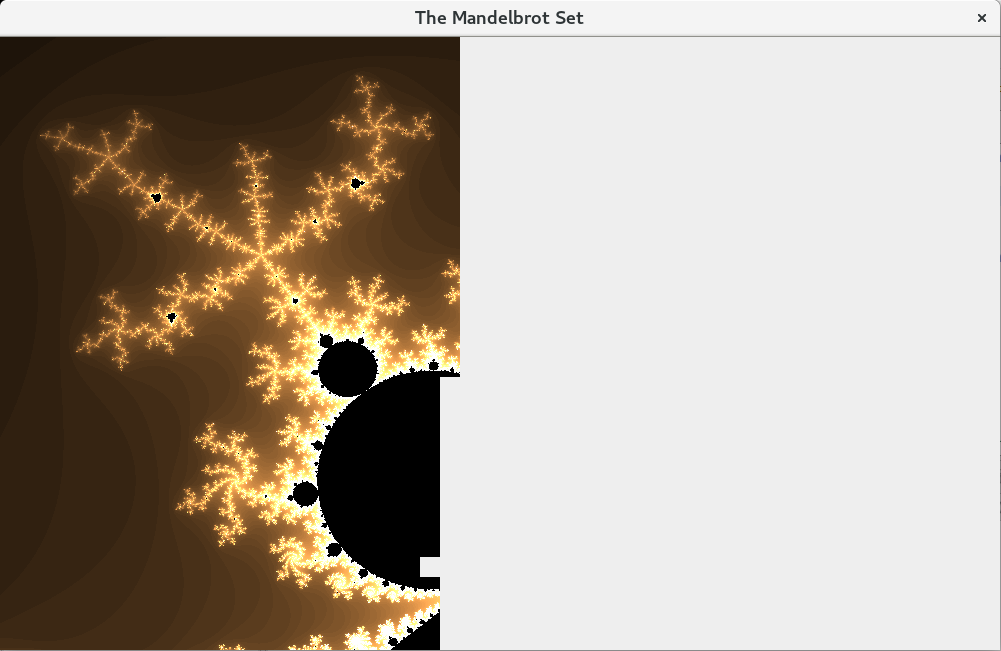
\includegraphics[width=.8\textwidth]{src/img/mandelbrot_running}
    \end{center}
  \caption{Capture d'écran en cours d'exécution, avec 10 threads.}
  \label{fig:running}
\end{figure}

\section{Travail à réaliser}

Le programme fourni inclut une classe \lstinline{SequentialDrawer}, qui contient une implémentation
séquentielle et bloquante de l'interface \lstinline{Drawer}.
Cette classe calcule à chaque rafraîchissement de la fenêtre l'image complète de l'ensemble de Mandelbrot,
en appelant successivement \lstinline{Area.getImage(function, palette)} pour chaque zone.
Le résultat est ensuite immédiatement affiché sur le canevas graphique par un appel
à \lstinline{area.drawImage(graphics, image)}.
Comme l'image est recalculée à chaque appel de \lstinline{draw}, cette implémentation est très lente,
mais elle constitue une base simple à partir de laquelle vous allez construire vos propres versions parallèles.
Votre but est de réimplémenter le serveur en suivant différentes stratégies.
Vous ne devez pas modifier cette classe, mais en créer de nouvelles
(par exemple \lstinline{AsyncDrawer}, \lstinline{PerAreaDrawer}, \lstinline{PoolDrawer}) qui implémentent la même interface.
La figure \ref{fig:running} montre une capture d'écran obtenue pendant l'exécution du programme après parallélisation.

Mesurez le temps d'exécution des différentes solutions, et tracez le graphe du temps nécessaire pour obtenir l'image complète en
fonction du nombre de threads (faites varier avec un pas de un entre un seul thread au total
jusqu'à environ 20 threads, puis vous pouvez espacer les mesures jusqu'à un thread par objet \lstinline{Area}).

Vous pouvez modifier les paramètres de la méthode \lstinline{Main.main()}
pour que les temps de calcul soient mieux adaptés à votre machine. Un temps autour de
30 secondes devrait convenir pour observer des effets intéressants.

\begin{enumerate}
\item Vous devez proposer une nouvelle implémentation de l'interface \lstinline{Drawer}
  dans laquelle le calcul de l'image doit être effectué une seule fois et dans un thread séparé.
  La méthode \lstinline{draw} doit retourner \lstinline{false} tant que l'image n'est pas prête,
  puis afficher l'image et retourner \lstinline{true} ensuite.

\item Même question, mais en parallélisant le calcul de l'image en lançant un thread par objet \lstinline{Area}.

\item Même question, mais en parallélisant le calcul de l'image en lançant un total de $n$ threads qui se répartissent les objets \lstinline{Area}.
\end{enumerate}

\end{document}
